% Draft 4: Springer LNCS template, as required by AIPR 2026 (proceedings in LNCS).
% Built from draft 3 (paper3/); sections are being rewritten one at a time.
% No page limit at AIPR 2026; length is driven by content.
\documentclass[runningheads]{llncs}

\usepackage[T1]{fontenc}
\usepackage{amsmath,amssymb}
\usepackage{graphicx}
\usepackage{booktabs}
\usepackage{xcolor}
\usepackage{subcaption}
\usepackage{url}
\usepackage{listings}
\usepackage{tikz}
\usetikzlibrary{arrows.meta,positioning,calc}
\usepackage[hidelinks]{hyperref}
\renewcommand\UrlFont{\color{blue}\rmfamily}

% Draft markers. Delete this block before submission; no marker may remain.
\newcommand{\verify}[1]{\textcolor{red}{[VERIFY: #1]}}

\lstset{basicstyle=\ttfamily\scriptsize, breaklines=true, columns=fullflexible, frame=single, xleftmargin=3pt, framexleftmargin=3pt, aboveskip=0pt, belowskip=0pt}

% Let pages carry more float material; the paper is figure-dense.
\setcounter{topnumber}{3}
\setcounter{totalnumber}{4}
\renewcommand{\topfraction}{0.9}
\renewcommand{\textfraction}{0.07}
\renewcommand{\floatpagefraction}{0.85}

\graphicspath{{figures/}}

\begin{document}

\title{Synthetic Video Generation for Robot Learning Using World Foundation Models}
\titlerunning{Synthetic Video Generation for Robot Learning}

\author{Shrey Jha \and Skyler Saucedo \and Frank Tanner}
\authorrunning{S. Jha et al.}

\institute{Innodata Inc.\\
\email{xxx@innodata.com}}

\maketitle

\begin{abstract}
A robot policy trained on a few egocentric recordings learns those recordings: one counter, one bucket, one light. Vision-language-action models cover that variety with hundreds of thousands of demonstrations, mostly the same tasks under new appearances, and recording them by hand is slow. Domain randomization is cheap but blind to the scene, giving a cleaning bucket textures no bucket has. We describe a pipeline on NVIDIA Cosmos that produces appearance variants of real clips while keeping the recorded actions. Cosmos 3 Nano reads a clip and writes an ontology: the task, each object with its box and role, and variations grounded in that role. GPT-4o mini rejects implausible candidates and writes the prompt. SAM2 turns the boxes into tracked masks, a subtraction step isolates the surface to repaint, and edge, depth, color and segmentation maps guide Cosmos Transfer 2.5. On 116 clips from 8 recordings, reasoning yields 72 admissible variations per clip in about two minutes, and one render takes 20 minutes on an A100; we rendered 64. Single-surface recolors preserve hand pose, object shape and motion, but the edit does not stay where it was sent: in the counter-wiping example the target region moves by a mean CIE76 $\Delta E$ of 75 and the protected region by 35, and cluttered scenes recolor almost entirely. Action-level variation with Cosmos Predict2 produced no motion. Appearance variation is now cheap to propose and render; containing the edit and generating new actions stand between this output and a robot training set.

\keywords{Synthetic data \and World foundation models \and NVIDIA Cosmos \and Egocentric video \and Robot learning.}
\end{abstract}

\section{Introduction}

Policies that generalize are trained on volumes of data no single lab records by hand. $\pi_0$ pretrains on more than 10,000 hours of robot data~\cite{pi0}; LingBot-VLA on about 20,000 hours from nine dual-arm platforms, with success rates still rising at that scale~\cite{lingbotvla}; EgoScale on 20,854 hours of egocentric human video, where action-prediction loss falls log-linearly with hours and that loss tracks success on a real robot~\cite{egoscale}. The last result is the one that matters here, because it makes egocentric human video rather than teleoperation the scalable source: a person wearing a camera while doing chores is training data. What the hours contain matters as much as how many there are. Lin et al.~\cite{lin2025scaling} collected 40,000 demonstrations and found that a single-task policy's generalization follows a power law in the number of training environments and objects, that additional demonstrations in the same environment stop helping past a threshold, and that 32 environments with one object each were enough for 90\% success in rooms and on objects never seen. The useful unit of data is a new combination of surface, object, lighting and clutter around the same action. We call that combination the ontology of a scene, and diversity of ontology, not hours, is what a policy needs.

\begin{figure}[t]
\centering
\begin{subfigure}{0.33\linewidth}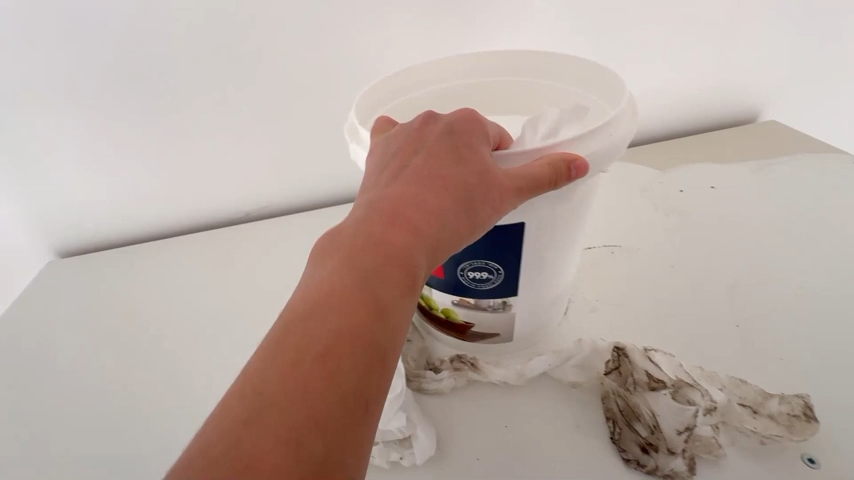
\includegraphics[width=\linewidth]{s03_original.png}\caption{what we started with}\end{subfigure}\hspace{2mm}
\begin{subfigure}{0.33\linewidth}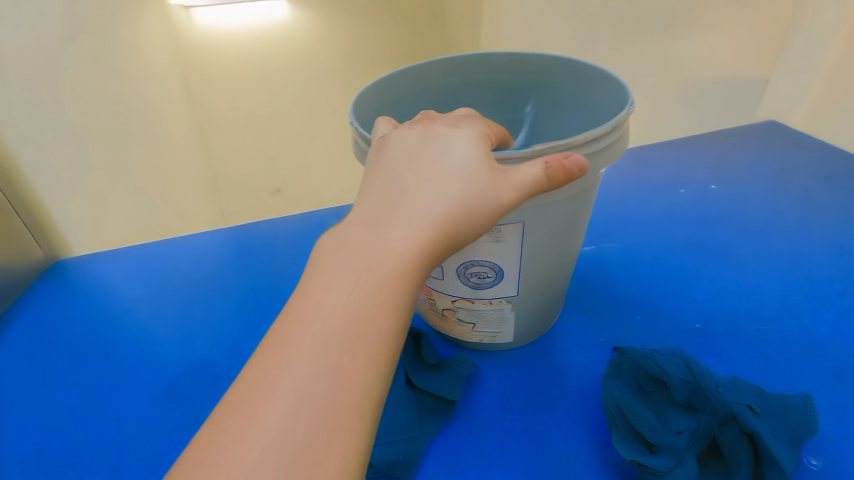
\includegraphics[width=\linewidth]{s04_created.png}\caption{what we created}\end{subfigure}
\caption{The running example. (a) A real clip: a person wiping a counter with a bucket and paper towels. (b) The variant rendered when asked to change only the countertop to blue. Counter color, hand pose, bucket geometry and motion are as intended; the beige wall, blue towels and bucket, and new ceiling light were not asked for.}
\label{fig:teaser}
\end{figure}

Recording that diversity is where the cost sits. An hour of egocentric video costs 8 to 15 USD in collector pay \verify{source for the hourly rate}, so 20,000 hours for a single task is 160,000 to 300,000 USD before anyone has found that many different kitchens, and the kitchens are the hard part: the scaling result says the next hour in the same room is close to worthless. The existing shortcuts each give up something. MimicGen multiplies 200 human demonstrations into 50,000 by replaying trajectory segments in new object poses, but in simulation and for robot trajectories, not video~\cite{mimicgen}. FieldGen automates the reaching phase of a demonstration and keeps the human for contact~\cite{fieldgen}; it saves operator time, not environments. Domain randomization perturbs colors and textures with no notion of the task, so a cleaning bucket gets a texture no bucket has~\cite{tobin2017}. Generative augmentation with image diffusion models produces plausible single frames but does not hold hands and objects steady across a clip~\cite{rosie,genaug}. Structure-conditioned video models can restyle a whole clip~\cite{gen1,controlnet}, and NVIDIA's Cosmos family packages this for physical AI~\cite{cosmos2025}, but none of them decides what in a clip should change and what must stay fixed.

We take the clip as the unit and permute the ontology around the recorded action. A reasoning model reads the clip and writes the scene as a structured ontology: the task, each object with its role in that task, and the variations each object could plausibly take while the task stays the same. A language model filters the candidates and writes a prompt, a segmenter builds a mask of the one surface to change, and a guided video-to-video model renders the variant with the hand motion intact (Fig.~\ref{fig:teaser}). On 116 clips from 8 recordings the reasoning stage admits 72 variations per clip, so a 15-second clip becomes 18 minutes of candidate video and a 10-minute recording about 4 hours, a 72-fold multiplier with no new recording and no new kitchen. The same arithmetic sets the limit: a render costs 20 minutes on one A100, or 80 GPU-hours per synthetic hour, so at today's speed the pipeline buys diversity rather than cheaper hours. For a robotics company the value is in the loop this closes. Real recordings from a deployment become synthetic variants the same day, the variants retrain the policy, the retrained policy goes back on the robot, and its new recordings seed the next round; the pipeline turns the real-to-sim-to-real cycle from a collection campaign into a batch job. The paper reports what the pipeline produces and where it stops. Single-surface recolors keep hand pose, object shape and motion, but the edit does not stay inside its mask: in the counter-wiping clip the protected region shifts by a mean CIE76 $\Delta E$ of 35 against 75 for the target. Scenes with many textures recolor wholesale, and two attempts at action-level change with Cosmos Predict2 returned the scene unchanged. Whether appearance diversity alone makes a policy more general, or whether action generation has to be solved first, is the question these results leave open.

\section{Background and Related Work}

World foundation models are video generators trained to respect physics, geometry and causality well enough to serve as simulators for robots~\cite{cosmos2025}. Cosmos releases three families: Predict forecasts future frames from text, an image or a video~\cite{cosmospredict2}; Transfer adapts a video across environments under multi-control conditioning on depth, segmentation, edge and blurred-RGB maps~\cite{cosmostransfer1,cosmos25}; Reason is a vision-language model for physical scene understanding~\cite{cosmosreason1}. Cosmos~3 folds the three into one omni-model with a reasoning tower and a generation tower~\cite{cosmos3}. Transfer descends from ControlNet~\cite{controlnet} and Gen-1~\cite{gen1}, which steer a frozen diffusion model with structure maps. The data problem is the one behind RT-2~\cite{rt2}, OpenVLA~\cite{openvla} and $\pi_0$~\cite{pi0}, all trained on the Open X-Embodiment pool~\cite{oxe}, and behind egocentric corpora such as Ego4D~\cite{ego4d}. Domain randomization~\cite{tobin2017} is the standard answer in simulation and is deliberately blind to semantics. ROSIE~\cite{rosie} and GenAug~\cite{genaug} let a language model decide what to vary and inpaint the result into robot images; we keep that premise, move it to video, where the edit must survive a moving hand, and make the decision explicit as a schema. Masks come from SAM2~\cite{sam2}, clip boundaries from TransNetV2~\cite{transnetv2}, and edges and depth from the Canny detector~\cite{canny1986} and a monocular depth network~\cite{depthanything} as packaged with Transfer.

\section{Method}
\label{sec:method}

Fig.~\ref{fig:pipeline} shows what goes in and what comes out: reasoning turns the clip into an ontology and candidate variations, guidance turns one variation into a prompt and four control maps, and generation renders it. The only manual decision is which variation to render. A clip is a frame sequence $V=\{I_t\}_{t=1}^{T}$ with $T=60$ at 4~fps and $854\times480$ pixels. The reasoning model $R$ maps the first frame to an ontology $\mathcal{O}=R(I_1)$: a task record, objects $\{o_k\}$ with normalized boxes $b_k\in[0,1000]^4$, and for each object candidate variations $\mathcal{U}_k$ such as ``solid blue matte.'' The prompt writer $L$ maps $(\mathcal{O},u)$ to a prompt $p$ for a chosen $u\in\mathcal{U}_k$; the segmenter $S$ maps a box and the clip to a tracked binary mask $S(b_k,V)\in\{0,1\}^{T\times H\times W}$; the generator $G$ maps $(V,p,\{c_j\},w)$ to a variant $V'$, where $c_j$ are control videos and $w$ their weights.

\begin{figure}[t]
\centering
\begin{tikzpicture}[
  font=\scriptsize,
  inbox/.style={draw, rounded corners=2pt, fill=black!4, text width=42mm, inner sep=3pt, align=left, minimum height=7mm},
  core/.style={draw, rounded corners=2pt, fill=green!12, text width=20mm, align=center, inner sep=3pt},
  outbox/.style={draw, rounded corners=2pt, fill=black!4, text width=33mm, align=center, inner sep=3pt},
  arr/.style={-{Latex[length=1.6mm]}, thick}
]
\node[inbox] (clip) {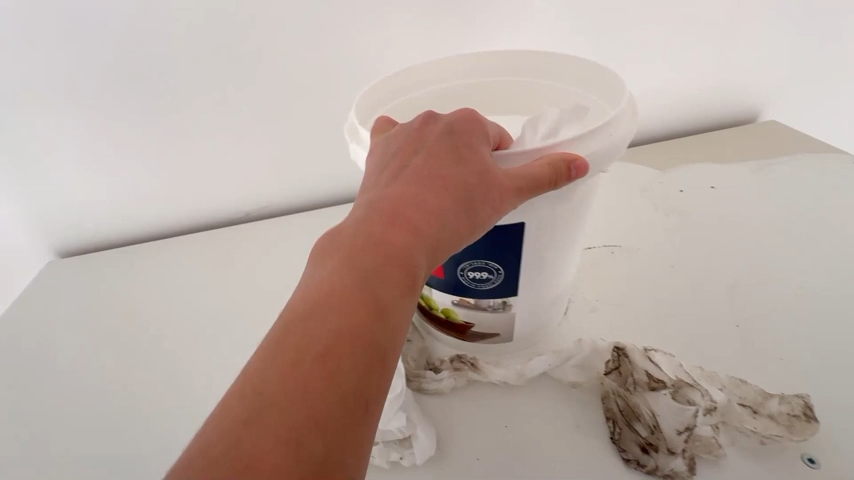
\includegraphics[height=6mm]{s03_original.png}\hspace{2pt}\begin{minipage}[b]{30mm}Original clip $V$\\60 frames, 4 fps\end{minipage}};
\node[inbox, below=1.5mm of clip] (prompt) {Ontology $\mathcal{O}$ + text prompt $p$};
\node[inbox, below=1.5mm of prompt] (maps) {Four guidance maps $c_j$: edges, depth, color, seg,\\with weights $w$ that balance them};
\node[inbox, below=1.5mm of maps] (mask) {Subtraction mask $M$: where the model should paint};
\node[core, right=7mm of $(prompt.east)!0.5!(maps.east)$] (tr) {\textbf{Cosmos Transfer 2.5}\\video-to-video generation};
\node[outbox, right=7mm of tr] (out) {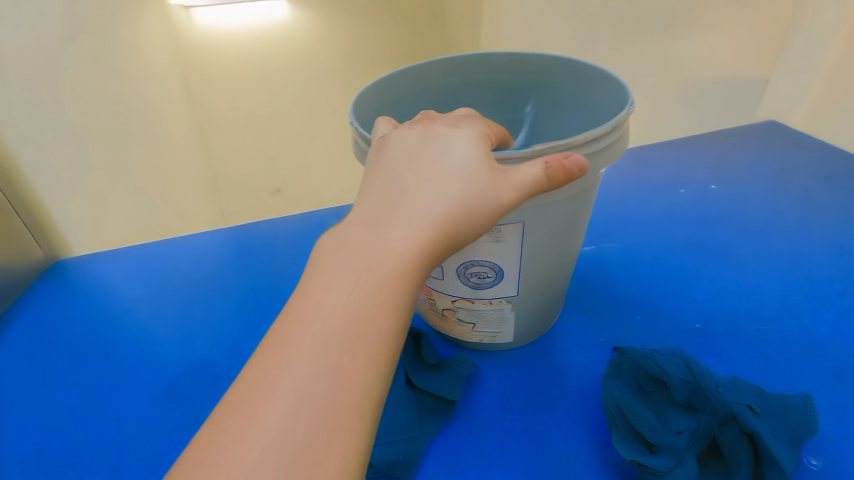
\includegraphics[width=30mm]{s04_created.png}\\Synthetic clip $V'$: same task, same actions, new appearance};
\coordinate (bus) at ($(clip.east)+(3.5mm,0)$);
\foreach \n in {clip,prompt,maps,mask} {\draw[thick] (\n.east) -- (\n.east -| bus);}
\draw[thick] (clip.east -| bus) -- (mask.east -| bus);
\draw[arr] (tr.west -| bus) -- (tr.west);
\draw[arr] (tr) -- (out);
\end{tikzpicture}
\caption{Pipeline. Every input to the renderer is produced by an earlier stage: the ontology and prompt by the reasoning model and the language model, the guidance maps by the preprocessors shipped with Transfer, and the mask by SAM2 from the ontology's boxes.}
\label{fig:pipeline}
\end{figure}

\subsection{Reasoning with Structured Ontologies}
\label{sec:reason}
Domain randomization swaps colors and textures at random and hopes the policy learns to ignore them. Our premise is that the model should first understand the scene, so that a bucket in a cleaning clip is a cleaning bucket and not a bucket on a shelf. We prompt the reasoning tower of Cosmos 3 Nano~\cite{cosmos3} (16B parameters, 8B in the tower) with the first frame and a fixed instruction asking for up to ten task-relevant objects with boxes and an exhaustive list of variations along seven dimensions per object (color, material, size, state, condition, interaction, brand). The answer is JSON in a fixed schema (Fig.~\ref{fig:ontology}). \texttt{role\_in\_task} conditions the variations on what the object is for; \texttt{robustness\_gaps} lists failure modes such as the bucket tipping over, which are changes of action and go to a different renderer (Sec.~\ref{sec:generation}). The raw count exceeds 100 per clip; 72 on average survive the filter below.

\begin{figure}[t]
\centering
\begin{minipage}[c]{0.31\linewidth}
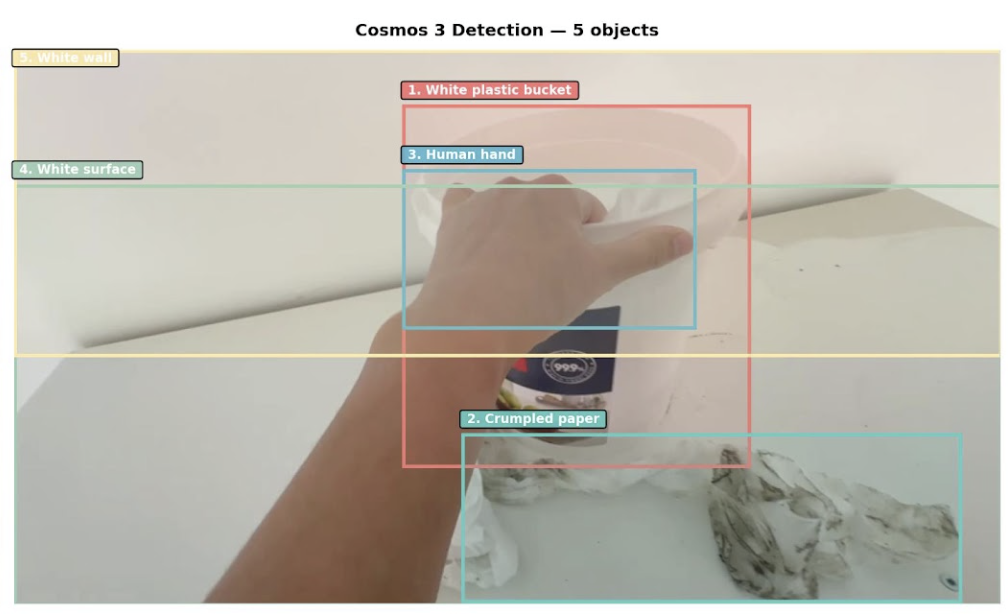
\includegraphics[width=\linewidth]{s08_detection.png}
\end{minipage}\hfill
\begin{minipage}[c]{0.67\linewidth}
\begin{lstlisting}
"task": { "name": "Disposing of crumpled paper into a bucket",
  "action_primitive": "Holding a bucket and positioning it" },
"key_objects": [{ "name": "White plastic bucket",
  "role_in_task": "Container for disposing of waste",
  "robustness_gaps": {
    "what_robot_must_handle": ["Different bucket sizes and shapes",
      "Labels with varying colors and designs", "Wet or slippery buckets"],
    "common_failure_modes": ["Bucket slips from hand",
      "Bucket tips over", "Bucket cannot be opened"] } }]
\end{lstlisting}
\end{minipage}
\caption{Reasoning output for the running example: five task-relevant objects with boxes, and an excerpt of the bucket's record. The task name is wrong (the clip shows wiping) and ``bucket cannot be opened'' is implausible for an open bucket; the filter stage exists to catch such entries.}
\label{fig:ontology}
\end{figure}

\subsection{From Ontology to Generation-Ready Prompts}
\label{sec:prompts}
GPT-4o mini~\cite{gpt4omini} keeps the variations that pass six plausibility checks (material against the task's contact forces, object size against the scene, material against the room type, physical possibility, lighting against time of day, and whether the object belongs in such a scene) and writes the Transfer prompt, which for the running example begins ``The video captures a person cleaning a solid blue countertop in a well-lit indoor kitchen\ldots\ The bucket and paper towels retain their original appearance.'' Three rules found by trial are encoded in the instruction: repeat the target attribute two or three times and name the material, not just the color; name every object that must stay unchanged; and describe the result as a scene rather than an edit, because Transfer was trained on captions of the output, not on instructions. Sec.~\ref{sec:leakage} measures how well the second rule holds.

\subsection{Guiding the Renderer}
\label{sec:guidance}
Transfer receives four control videos, each protecting a different part of the source (Fig.~\ref{fig:maps}, top). Canny edges $c_{\mathrm{edge}}$~\cite{canny1986} keep the shapes, so the bucket stays a bucket; monocular depth $c_{\mathrm{depth}}$~\cite{depthanything} keeps the layout; a heavily blurred copy of the source $c_{\mathrm{vis}}$ keeps the palette and lighting; a segmentation video $c_{\mathrm{seg}}$ says where to paint. The first three come from the preprocessors shipped with Transfer. The fourth needs one extra step, because the surface to recolor overlaps the bucket, towels and hand that must not change. SAM2~\cite{sam2} returns a tracked mask for the surface box $b_{\mathrm{surf}}$, which includes whatever lies on the counter, and one for each object box $b_k$; the final mask is
\begin{equation}
    M_t = S(b_{\mathrm{surf}},V)_t \;\setminus\; \bigcup_{k} S(b_k,V)_t ,
    \label{eq:mask}
\end{equation}
computed per frame on SAM2's propagated masks, so $M$ is temporally consistent without a separate tracker (Fig.~\ref{fig:maps}, bottom). $M$ enters Transfer as $c_{\mathrm{seg}}$. It is a control signal, not painter's tape: the model follows it to the degree set by the seg weight, and nothing forbids change outside $M$. The weights $w$ are the one set of hyperparameters we tuned, by moving each until a failure appeared and backing off (Table~\ref{tab:weights}). Edges matter most and are pinned on both sides; color guidance must be nearly off, because it conditions on the source colors and opposes any recolor.

\begin{figure}[t]
\centering
\begin{subfigure}{0.24\linewidth}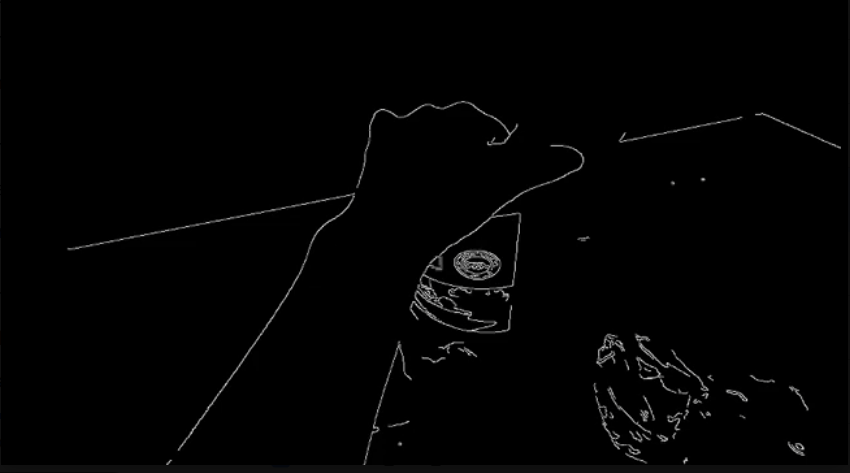
\includegraphics[width=\linewidth]{s10_edges.png}\caption{edges}\end{subfigure}\hfill
\begin{subfigure}{0.24\linewidth}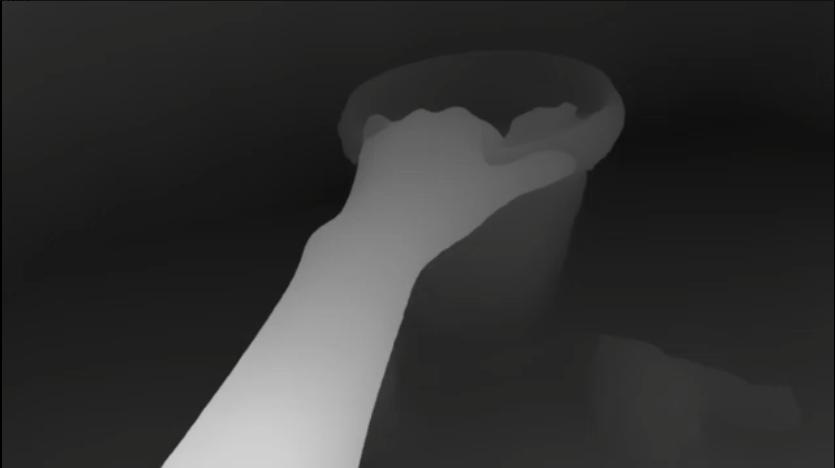
\includegraphics[width=\linewidth]{s10_depth.png}\caption{depth}\end{subfigure}\hfill
\begin{subfigure}{0.24\linewidth}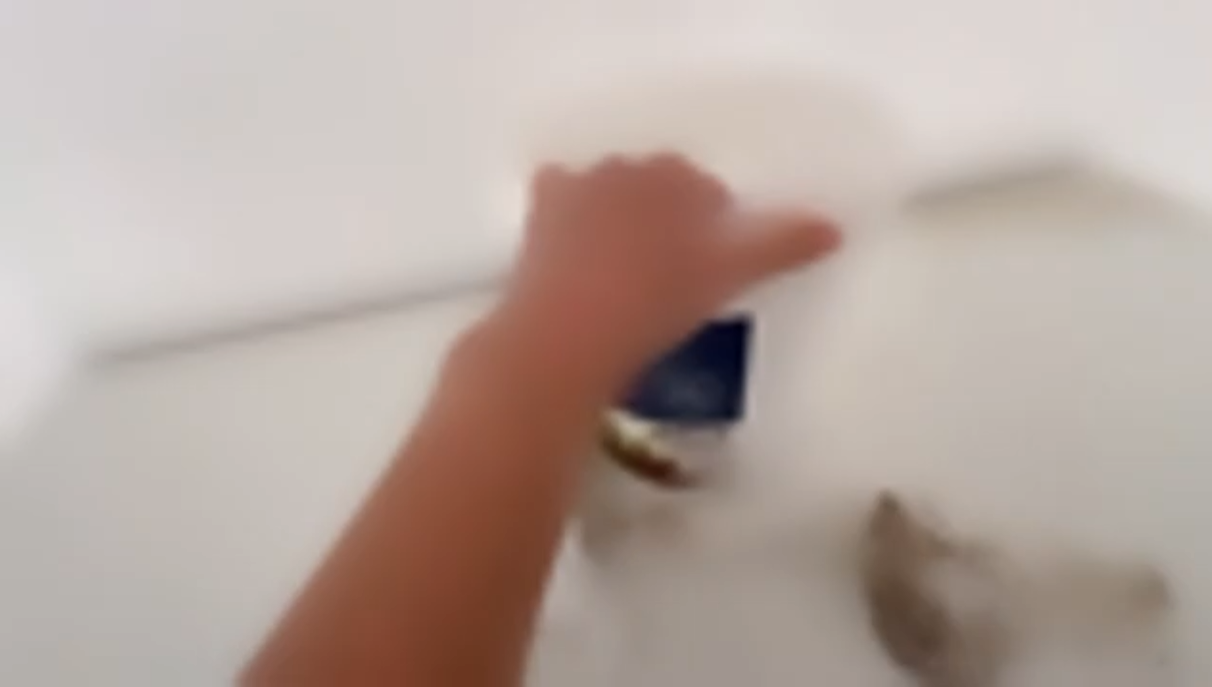
\includegraphics[width=\linewidth]{s10_color.png}\caption{color (vis)}\end{subfigure}\hfill
\begin{subfigure}{0.24\linewidth}
\includegraphics[width=\linewidth]{s10_mask.png}\caption{mask (seg)}\end{subfigure}\\[1.5mm]
\begin{subfigure}{\linewidth}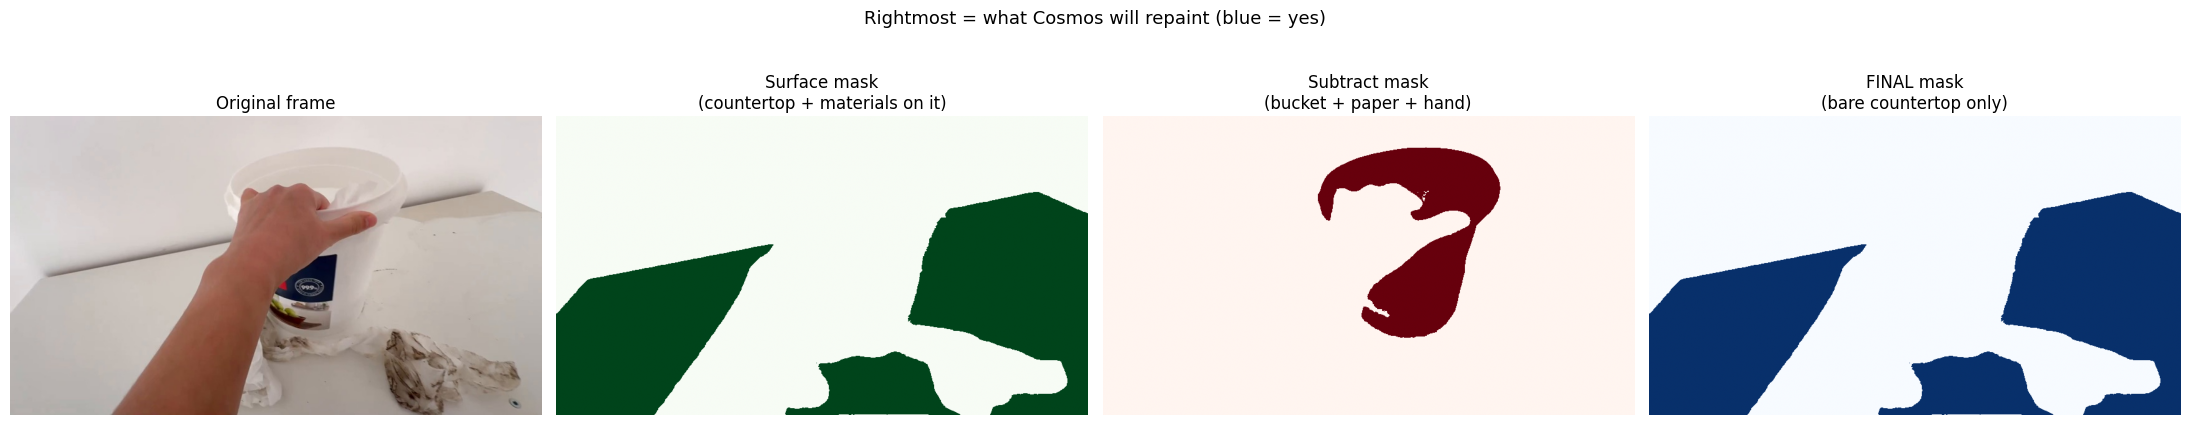
\includegraphics[width=\linewidth]{s11_mask_strip.png}\caption{building the subtraction mask}\end{subfigure}
\caption{Top: the four guidance maps for one frame. Edges keep the shapes, depth keeps the layout, color keeps the lighting, and the mask says where to paint. Bottom, left to right: original frame; SAM2 surface mask, which includes the materials on the counter; union of the bucket, paper and hand masks; final mask $M$ of Eq.~\ref{eq:mask}. Blue marks what the renderer is meant to repaint.}
\label{fig:maps}
\end{figure}

\begin{table}[t]
\centering
\caption{Control weights for Cosmos Transfer~2.5 as passed to the model (they sum to 0.9) and the failure that bounds each.}
\label{tab:weights}
\small
\begin{tabular}{@{}lrll@{}}
\toprule
Control & Weight & Too low & Too high \\
\midrule
edge  & 0.5   & objects lose shape & nothing changes \\
depth & 0.2   & layout drifts & scene flattens to a plane \\
vis (color) & 0.025 & none observed & recolor reverts \\
seg (mask)  & 0.175 & edits unlocalized & over-constrained \\
\bottomrule
\end{tabular}
\end{table}

\subsection{Generation}
\label{sec:generation}
Cosmos Transfer~2.5~\cite{cosmos25} renders $V'=G(V,p,\{c_j\},w)$ with 35 denoising steps and guidance scale 4; at 2 and 3 it often ignored the variation, and above 5 it followed the prompt but lost the room. Seeds were not fixed; outputs are 60 frames at $854\times480$ and 4~fps. Transfer preserves the source motion by construction, so action-level entries such as ``bucket tips over'' go to Cosmos Predict2 (2B, Video2World)~\cite{cosmospredict2}, which forecasts frames from a conditioning clip and a description of what happens next.

\section{Results}
\label{sec:results}

\paragraph{Setup}
One person recorded 8 egocentric videos of household chores (counter wiping, cloth folding, bed making, cable wrapping), about 10 minutes each. TransNetV2~\cite{transnetv2} split them into 116 clips of at most 15~s at 4~fps and $854\times480$, about 30 minutes in total. All runs used one A100 80~GB. Per clip, reasoning took 130~s, a Transfer render 20~min and a Predict2 render 3.5~min; GPT-4o mini for all 116 clips cost about 0.12 USD. We ran reasoning on all 116 clips and rendered 64 Transfer variants of 10 source clips plus two Predict2 clips; at these rates the 116 clips could become $116\times72 = 8{,}352$ variants at about 2{,}800 A100-hours. No policy was trained on the output.

\subsection{Appearance Variation}
Fig.~\ref{fig:teaser} is the running example under the blue-countertop prompt. The counter is blue, hand pose and bucket geometry are preserved frame for frame, and the motion is the source motion. Every unintended change is also easy to see: the rags became blue cloth, the bucket grey-blue, the wall beige, and a ceiling fixture appeared, although the prompt named the bucket, towels and lighting as preserved. Fig.~\ref{fig:more}a,b shows the cloth-folding clip, where the prompt asked for a cobalt blanket on the left of the bed and the render turned nearly every surface blue. Where the counter clip leaks at the edges of the target, a frame with many textures fails almost completely. Fig.~\ref{fig:more}c,d show a blue-desk prompt whose color spreads onto the shelf objects and the cable, and a navy-rug prompt that returned the right bedspread with smeared surfaces and a warped hand, the shape-collapse failure of Table~\ref{tab:weights}.

\begin{figure}[t]
\centering
\begin{subfigure}[t]{0.30\linewidth}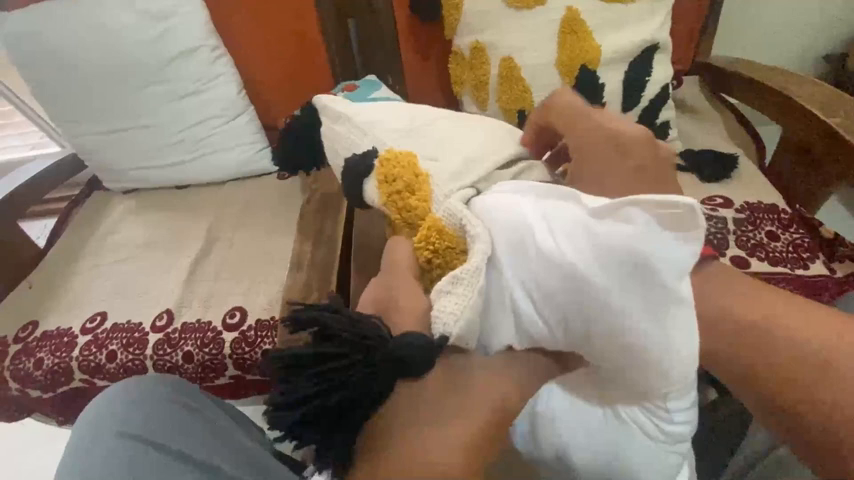
\includegraphics[width=\linewidth]{s14_old.png}\caption{cloth folding, source}\end{subfigure}\hspace{2mm}
\begin{subfigure}[t]{0.30\linewidth}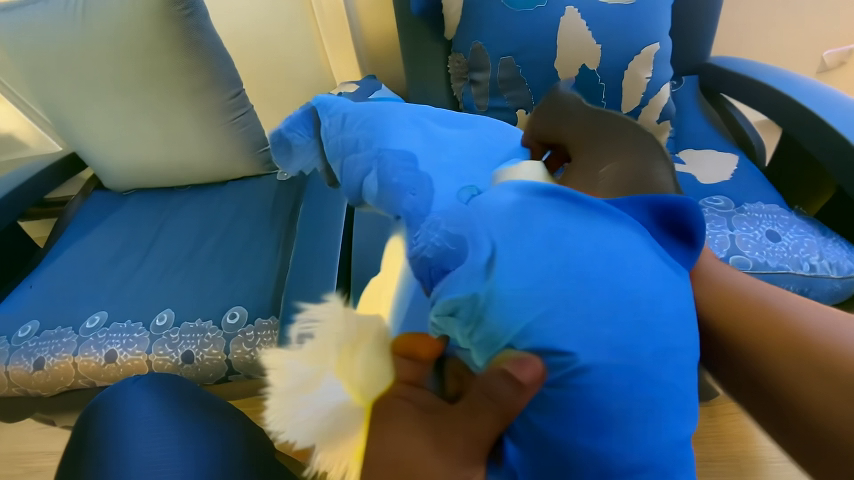
\includegraphics[width=\linewidth]{s14_new.png}\caption{cobalt blanket prompt}\end{subfigure}\\[1.5mm]
\begin{subfigure}[t]{0.105\linewidth}\centering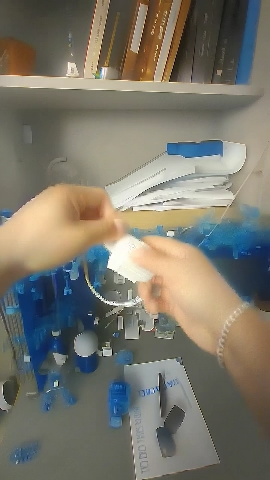
\includegraphics[height=1.6cm]{s16_left.png}\caption{}\end{subfigure}\hfill
\begin{subfigure}[t]{0.29\linewidth}\centering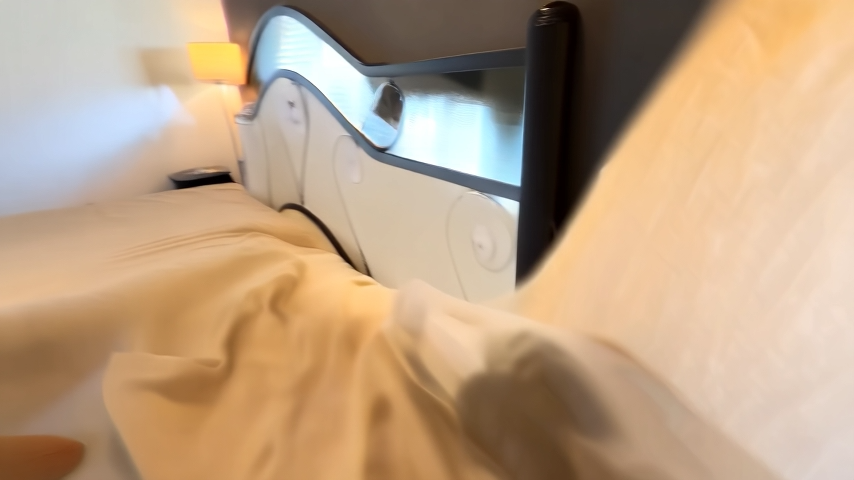
\includegraphics[height=1.6cm]{s16_middle.png}\caption{}\end{subfigure}\hfill
\begin{subfigure}[t]{0.29\linewidth}\centering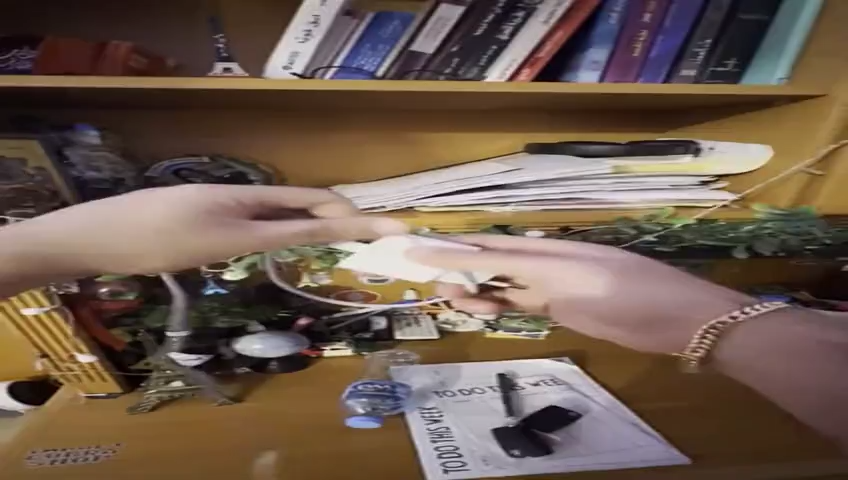
\includegraphics[height=1.6cm]{s15_generated.png}\caption{}\end{subfigure}\hfill
\begin{subfigure}[t]{0.29\linewidth}\centering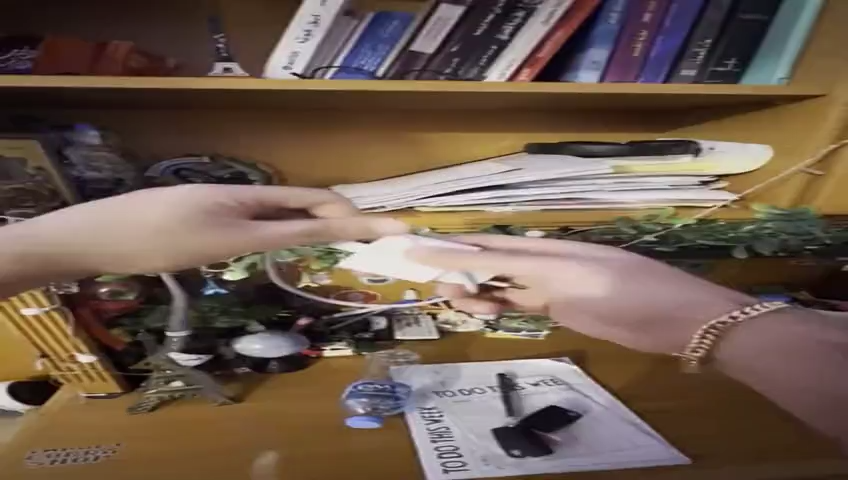
\includegraphics[height=1.6cm]{s16_right.png}\caption{}\end{subfigure}
\caption{Where the renders fail. (a, b) The prompt targeted one blanket; the render recolored cushions, chair and cloth. (c) Blue desk: color spreads onto the shelf objects and cable. (d) Navy-rug prompt: the bedspread is right, surfaces smear and the hand warps. (e, f) Predict2 cable-wrapping and paper-rotation prompts: nothing moves.}
\label{fig:more}
\end{figure}

\subsection{Measuring Leakage}
\label{sec:leakage}
To put a number on the unintended change we compare source and variant frame by frame in CIELAB and split the per-pixel CIE76 distance $\Delta E$ by the tracked mask $M$; a $\Delta E$ of 10 is unmistakable to a viewer. Table~\ref{tab:leakage} gives the result for the counter clip, the one render with a usable tracked mask. The target moved by a mean $\Delta E$ of 75, so the recolor worked. The protected region moved by 35, 95\% of its pixels moved by more than 10, and the chroma-only distance shows the change is color rather than exposure. The seg control and the prompt's preservation clause were the two soft mechanisms for containment, and neither was sufficient.

\begin{table}[t]
\centering
\caption{Masked color difference for the counter-wiping variant over 60 frames; each region covers about half the frame. The protected region changes by almost half as much as the target, and nearly all of it changes visibly.}
\label{tab:leakage}
\small
\begin{tabular}{@{}lrr@{}}
\toprule
 & Target ($M$) & Protected ($\bar M$) \\
\midrule
Mean $\Delta E$ & 75.5 & 34.8 \\
Mean chroma-only $\Delta E$ ($a$, $b$ channels) & 68.2 & 24.2 \\
Pixels with $\Delta E > 10$ (\%) & -- & 94.5 \\
Pixels with $\Delta E > 20$ (\%) & -- & 65.3 \\
\bottomrule
\end{tabular}
\end{table}

\subsection{Action-Level Variation}
\label{sec:action}
Two action variations from the ontology were run through Predict2 (35 steps, $848\times480$, 93 frames at 16~fps): winding a charger cable around its block with the block held fixed, and a sheet of paper rotating 90 degrees while the objects on it stay put. In both renders the forecast reproduces the conditioning scene and the cable and paper do not move (Fig.~\ref{fig:more}e,f). The model held the scene stable, a kind of success for a world model, and did not perform the action, the only thing we asked of it.

\section{Closing the Gap}
\label{sec:gap}

Everything above is about rendered video; nothing is about a robot. The claim that appearance variants improve policy generalization is the premise of this work, and the honest reading of Table~\ref{tab:leakage} is that today's variants would teach a policy that counters, towels and buckets change color together. Training a policy on them and measuring held-out success is the experiment that decides whether the pipeline is useful, and it is the top item on our list.

The containment failure has a specific cause: the mask entered the renderer only as a soft control, and the preservation clause is a request. Transfer~1 supports spatiotemporal control-weight maps~\cite{cosmostransfer1}, and compositing source pixels back outside $M$ after rendering is trivial; either should cut the protected-region $\Delta E$ by a large factor. The tracked masks retained for the desk and cloth-folding renders cover under 1\% and about 2\% of the frame; if those are the masks Transfer received, SAM2's propagation collapsed, which would explain Fig.~\ref{fig:more}b, and a pipeline that depends on a tracked mask needs a coverage check before rendering. The ontology is a strong proposal generator with an unmeasured error rate (Fig.~\ref{fig:ontology}), and we compare against no baseline; a prompt-level version of domain randomization, with the same target and controls but color and material drawn at random, would test our third claim cheaply. The weights in Table~\ref{tab:weights} were tuned on one clip and checked on three, all from one home.

Two paths lead to action-level data. Predict2 lacks the contact physics the cable and paper prompts require; fine-tuning it on real manipulation video with low-rank adapters is the direct route. The longer bet is Cosmos~3, which collapses the pipeline into one reasoning tower and one generation tower trained with spatial grounding~\cite{cosmos3}; its Nano variant already serves as our reasoner, but its generation tower did not support video-to-video transfer when we tried it.

\section{Conclusion}
A pipeline on NVIDIA Cosmos turns an egocentric clip into task-grounded appearance variations in about two minutes and renders one with the source motion intact in about twenty, so a small dataset becomes thousands of candidate clips at the price of GPU time. Appearance changes work for simple scenes; cluttered scenes and action-level changes remain unsolved, and the edit does not stay inside the mask. Whether synthetic appearance data alone makes a policy more general, or whether action generation must be solved first, is the question this pipeline now makes it possible to ask.


\bibliographystyle{splncs04}
\bibliography{refs}

\end{document}
